\begin{figure}[t]
%\centerline{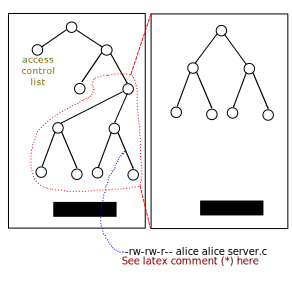
\includegraphics{fig/commitcheckout.pdf}}
\caption{The figure shows the result of a checkout and commit command.
Part (a) shows the original HEAD of the repository. The user checks out that
HEAD at the relative point, and copies it out as part (b). The user then
modifies it to part (c). After that the user make a commit back to the
repository, and the repository stores part (d). \hw{Current graph is a fake one.
    TODO draw the graph.}
}

\label{f:checkout-commit}
\end{figure}

\endinput


